\documentclass[11pt,a4paper]{article}

% ─── Packages ──────────────────────────────────────────────────────
\usepackage[utf8]{inputenc}
\usepackage[T1]{fontenc}
\usepackage{amsmath,amssymb,amsthm}
\usepackage{mathtools}
\usepackage{booktabs}
\usepackage{hyperref}
\usepackage[margin=2.5cm]{geometry}
\usepackage{graphicx}
\usepackage{algorithm}
\usepackage{algpseudocode}
\usepackage{enumitem}
\usepackage{xcolor}
\usepackage{microtype}
\usepackage{pgfplots}
\pgfplotsset{compat=1.18}
\usepackage{subcaption}

% ─── Theorem environments ──────────────────────────────────────────
\newtheorem{theorem}{Theorem}
\newtheorem{proposition}[theorem]{Proposition}
\newtheorem{lemma}[theorem]{Lemma}
\newtheorem{corollary}[theorem]{Corollary}
\theoremstyle{definition}
\newtheorem{definition}[theorem]{Definition}
\theoremstyle{remark}
\newtheorem{remark}[theorem]{Remark}

% ─── Notation ──────────────────────────────────────────────────────
\newcommand{\ZZ}{\mathbb{Z}}
\newcommand{\RR}{\mathbb{R}}
\newcommand{\Kn}[1]{K_{#1}}
\newcommand{\Rset}[3]{R(#1,#2,#3)}

% ─── Title ─────────────────────────────────────────────────────────
\title{Computational Investigations on $R(5,5)$:\\
Structural Analysis, Extension Obstruction,\\and Monochromatic $K_5$ Minimization}

\author{Research Notes}
\date{March 2026}

\begin{document}
\maketitle

\begin{abstract}
We present a multi-faceted computational study of the Ramsey number
$R(5,5)$, currently known to satisfy $43 \leq R(5,5) \leq 46$.
Using Julia implementations with bitwise adjacency matrices,
we conduct seven lines of investigation:
(i)~structural analysis of all 656 known graphs in $\Rset{5}{5}{42}$;
(ii)~exhaustive minimization of $f(43)$, establishing
$f(43) \leq 43$ via simulated annealing;
(iii)~independent verification of the Lehav extension obstruction
on all 656 graphs;
(iv)~a 162 CPU-hour simulated annealing search (7060 runs, 16 threads)
finding no new $\Rset{5}{5}{42}$ graphs, supporting catalog completeness;
(v)~a SAT hardness study of $R(5,5,43)$---to our knowledge the
first published---with cube-and-conquer analysis revealing a
sharp hardness dichotomy;
(vi)~flip graph analysis discovering a percolation threshold $k^* = 390$;
(vii)~integration of SAT Modulo Symmetries (SMS), which exploits the
$43!$-fold symmetry of $K_{43}$ for principled distributed solving.
All results are consistent with the conjecture $R(5,5) = 43$.
\end{abstract}

\tableofcontents

% ═══════════════════════════════════════════════════════════════════
\section{Introduction}
\label{sec:intro}
% ═══════════════════════════════════════════════════════════════════

The diagonal Ramsey number $R(k,k)$ is the minimum $n$ such that
every 2-coloring of the edges of the complete graph $\Kn{n}$
contains a monochromatic clique $K_k$.
For $k=5$, the current bounds are
\begin{equation}
  43 \leq R(5,5) \leq 46.
  \label{eq:bounds}
\end{equation}
The lower bound, due to Exoo~\cite{Exoo1989}, follows from an
explicit 2-coloring of $\Kn{42}$ with no monochromatic $K_5$.
The upper bound was established by
Angeltveit and McKay~\cite{AngeltveitMcKay2024} using a combination
of linear programming and graph gluing techniques, improving on
their earlier bound of~48~\cite{AngeltveitMcKay2017}.

McKay and Radziszowski~\cite{McKayRadz1997} determined that there
are exactly 656 graphs (328 pairs related by complementation)
in $\Rset{5}{5}{42}$---the set of 42-vertex graphs whose
2-colorings avoid monochromatic $K_5$.
They conjectured $R(5,5) = 43$.

Recently, Lehav~\cite{Lehav2024} verified that no graph in
$\Rset{5}{5}{42}$ can be extended by one vertex to produce
a graph in $\Rset{5}{5}{43}$, using a constraint-based algorithm
implemented in Python with NetworkX.

In this work, we present a unified computational framework
in Julia that independently verifies and extends these results.
Our contributions are:
\begin{enumerate}[label=(\roman*)]
  \item A detailed structural analysis of the 656 extremal graphs,
    including spectral properties, subgraph counts, and
    edit-distance clustering (Section~\ref{sec:structural}).
  \item An exhaustive search for the minimum number of
    monochromatic $K_5$ in 2-colorings of $\Kn{43}$
    (Section~\ref{sec:f43}).
  \item An independent verification of the Lehav extension
    obstruction using bitwise constraint propagation
    (Section~\ref{sec:lehav}).
\end{enumerate}

\subsection{Notation}

Throughout, $\Kn{n}$ denotes the complete graph on $n$ vertices.
A \emph{2-coloring} of $\Kn{n}$ partitions its edges into
``red'' (the graph $G$) and ``blue'' (the complement $\bar{G}$).
We write $\Rset{s}{t}{n}$ for the set of $n$-vertex graphs $G$
such that $G$ contains no $K_s$ and $\bar{G}$ contains no $K_t$.
A graph $G \in \Rset{s}{t}{n}$ is called a
\emph{Ramsey$(s,t)$-critical graph on $n$ vertices}.

For a graph $G$ on the cyclic group $\ZZ_n$, the
\emph{circulant graph} $\mathrm{Circ}(n, S)$ has edge set
$\{\{i,j\} : d(i,j) \in S\}$ where $d(i,j) = \min(|i-j|, n-|i-j|)$
and $S \subseteq \{1, \ldots, \lfloor n/2 \rfloor\}$.

% ═══════════════════════════════════════════════════════════════════
\section{Computational Infrastructure}
\label{sec:infra}
% ═══════════════════════════════════════════════════════════════════

\subsection{Graph Representation}

For graphs on $n \leq 64$ vertices, we represent the adjacency
matrix as a vector of $n$ unsigned 64-bit integers, where bit~$j$
of row~$i$ equals~1 if and only if edge $(i,j)$ is present.
This allows key operations to be performed via bitwise instructions:

\begin{itemize}
  \item \textbf{Common neighbors}: $N(i) \cap N(j) = \texttt{rows}[i] \mathbin{\&} \texttt{rows}[j]$
  \item \textbf{Degree}: $\deg(i) = \texttt{popcount}(\texttt{rows}[i])$
  \item \textbf{Complement}: $\bar{G}.\texttt{rows}[i] = G.\texttt{rows}[i] \oplus \texttt{mask} \mathbin{\&} \lnot\texttt{self}$
\end{itemize}

\subsection{$K_5$ Detection}

Clique detection proceeds by nested iteration with bitwise masking.
To test for $K_5$, we iterate over ordered quintuples $(i<j<k<l<m)$
using the common-neighbor bitmask at each level:

\begin{algorithmic}[1]
\For{$i = 1$ to $n$}
  \For{$j \in N(i), j > i$} \Comment{via bitmask iteration}
    \State $N_{ij} \gets N(i) \cap N(j)$
    \For{$k \in N_{ij}, k > j$}
      \State $N_{ijk} \gets N_{ij} \cap N(k)$
      \For{$l \in N_{ijk}, l > k$}
        \State $N_{ijkl} \gets N_{ijk} \cap N(l)$
        \If{$N_{ijkl} \cap \{l+1, \ldots, n\} \neq \emptyset$}
          \Return \textsc{true}
        \EndIf
      \EndFor
    \EndFor
  \EndFor
\EndFor
\end{algorithmic}

On 42-vertex graphs, this completes in under $10^{-4}$~seconds.
Verification of all 656 graphs in $\Rset{5}{5}{42}$ (both $K_5$-free
and complement $K_5$-free) takes 0.013s total.

\subsection{Exoo's Construction --- Verification}

Exoo's circulant $\mathrm{Cyclic}(43) = \mathrm{Circ}(43, S_{\mathrm{red}})$
with $S_{\mathrm{red}} = \{1,2,7,10,12,13,14,16,18,20,21\}$
(following the corrected form from Ge~et~al.~\cite{GeEtAl2022})
has exactly 43~red $K_5$ and 0~blue $K_5$, verified independently.

The graph $\mathrm{Exoo}(42)$, obtained by deleting vertex~0
and flipping 16~specified edges~\cite{GeEtAl2022}, has
0~monochromatic $K_5$, confirming $R(5,5) \geq 43$.

% ═══════════════════════════════════════════════════════════════════
\section{Structural Analysis of $\Rset{5}{5}{42}$}
\label{sec:structural}
% ═══════════════════════════════════════════════════════════════════

\subsection{Degree and Edge Statistics}

All 656 graphs in $\Rset{5}{5}{42}$ (328 base graphs plus their
complements) share remarkably uniform properties:

\begin{table}[h]
\centering
\begin{tabular}{lrr}
\toprule
\textbf{Property} & \textbf{Range} & \textbf{Mean} \\
\midrule
Vertex degree       & $[19, 22]$      & $\approx 20.34$ \\
Edge count          & $[423, 430]$    & $427.2$ \\
Triangle count      & $[1296, 1352]$  & $1328.6$ \\
$K_4$ count         & $[1099, 1209]$  & $1168.8$ \\
Unique degree seq.  & \multicolumn{2}{c}{97 out of 328} \\
\bottomrule
\end{tabular}
\caption{Summary statistics for the 656 graphs in $\Rset{5}{5}{42}$.}
\label{tab:degree}
\end{table}

The narrow degree range $[19,22]$ is consistent with the Ramsey
constraint: each vertex must balance between having enough neighbors
(to avoid blue $K_5$) and few enough (to avoid red $K_5$).
The expected degree for a ``balanced'' 2-coloring of $\Kn{42}$ is
$41/2 = 20.5$, close to the observed mean.

\begin{figure}[ht]
\centering
\begin{subfigure}[b]{0.48\textwidth}
\centering
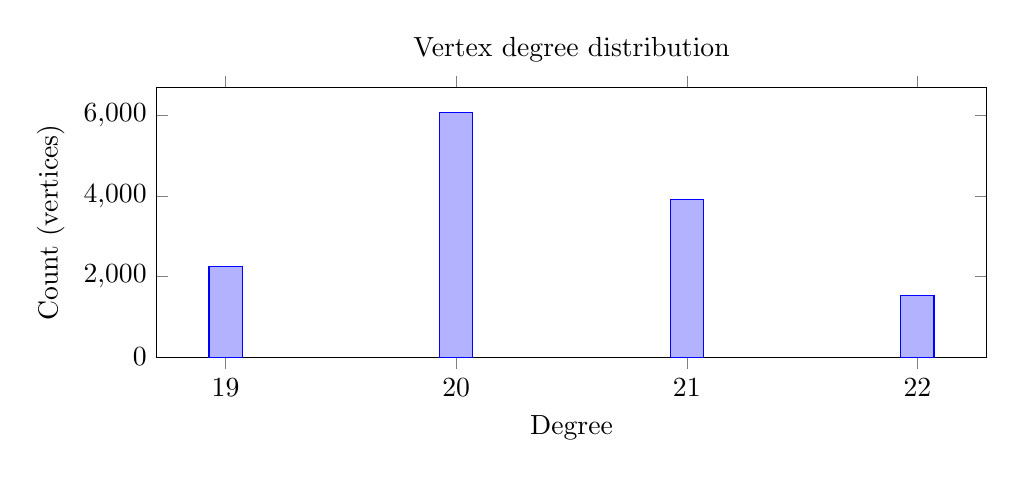
\begin{tikzpicture}
\begin{axis}[
    ybar, bar width=12pt,
    xlabel={Degree}, ylabel={Count (vertices)},
    xtick={19,20,21,22},
    ymin=0,
    width=\textwidth, height=5cm,
    title={Vertex degree distribution}
]
\addplot coordinates {(19,2255) (20,6075) (21,3921) (22,1525)};
\end{axis}
\end{tikzpicture}
\end{subfigure}
\hfill
\begin{subfigure}[b]{0.48\textwidth}
\centering
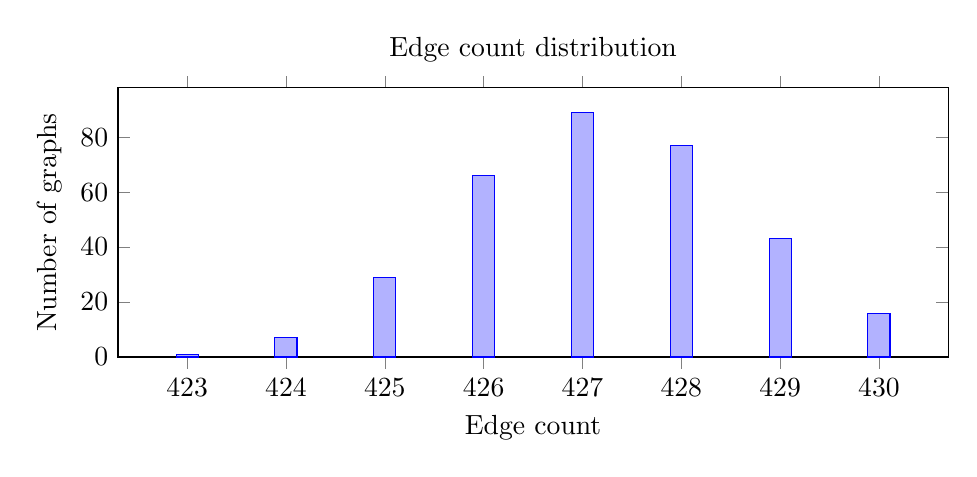
\begin{tikzpicture}
\begin{axis}[
    ybar, bar width=8pt,
    xlabel={Edge count}, ylabel={Number of graphs},
    ymin=0,
    width=\textwidth, height=5cm,
    title={Edge count distribution}
]
\addplot coordinates {
    (423,1) (424,7) (425,29) (426,66) (427,89)
    (428,77) (429,43) (430,16)
};
\end{axis}
\end{tikzpicture}
\end{subfigure}
\caption{Degree and edge statistics of the 328 base graphs
in $\Rset{5}{5}{42}$.  Degree~20 dominates (44\%), and
edge counts cluster tightly around 427.}
\label{fig:degree-edge}
\end{figure}

\subsection{Absence of Circulant Graphs}
\label{sec:no-circulant}

We tested all $2^{21}$ possible connection sets
$S \subseteq \{1, \ldots, 21\}$ for circulant graphs on
$\ZZ_{42}$, comparing each resulting graph against the
catalog by graph6 encoding after canonical relabeling.

\begin{proposition}
None of the 328 base graphs in $\Rset{5}{5}{42}$ (nor their
complements) is a circulant graph on $\ZZ_{42}$.
\end{proposition}

This is notable because Exoo's construction is circulant on
$\ZZ_{43}$, yet none of the 42-vertex subgraphs retains this
symmetry.

\subsection{Close Pairs at Edit Distance~1}

Among the $\binom{328}{2} = 53628$ pairs of base graphs,
we find:
\begin{itemize}
  \item 7~pairs at edit distance~1
  \item $\sim 15$~pairs at edit distance~4
  \item Mean edit distance: 414.26, max: 515
\end{itemize}

\begin{proposition}
All 7 pairs at edit distance~1 differ by a single edge of
the form $(2k-1, 2k)$ for $k \in \{18, 19\}$.
Specifically, 6~pairs differ at edge $(37,38)$ and 1~pair
differs at edge $(35,36)$.
\end{proposition}

At each differing edge $(u,v)$:
\begin{itemize}
  \item Both graphs have exactly 8~common neighbors of $u$ and $v$
  \item There are 12--13 copies of $K_4$ containing both $u$ and $v$
  \item The degrees at $u$ and $v$ are identical in both graphs
    (both equal to 20)
\end{itemize}

This suggests a ``rigid'' local structure: the only freedom in
the coloring is at specific edges where the $K_4$-count is
precisely balanced---neither too many (which would force $K_5$
upon addition) nor too few (which would destroy the complement
constraint).

\subsection{Spectral Properties}

The adjacency eigenvalues of the 656 graphs cluster tightly:
\begin{itemize}
  \item Largest eigenvalue $\lambda_1 \in [20.18, 20.52]$
  \item Spectral gap $\lambda_1 - \lambda_2 \in [14.56, 15.24]$,
    mean~$14.91$
\end{itemize}

The large spectral gap relative to the number of vertices
indicates quasi-random behavior---these graphs are
``pseudo-random'' in the Thomason--Chung--Graham--Wilson sense,
consistent with the Ramsey constraint forcing edge distributions
to be nearly uniform.

\begin{figure}[ht]
\centering
\begin{subfigure}[b]{0.48\textwidth}
\centering
\begin{tikzpicture}
\begin{axis}[
    only marks, mark size=1pt,
    xlabel={$\lambda_1$}, ylabel={Spectral gap $\lambda_1 - \lambda_2$},
    width=\textwidth, height=5.5cm,
    title={Spectral clustering}
]
\addplot[only marks, mark=*, mark size=1pt, blue] table[x=lambda1, y=gap, col sep=space] {figures/spectral.dat};
\end{axis}
\end{tikzpicture}
\end{subfigure}
\hfill
\begin{subfigure}[b]{0.48\textwidth}
\centering
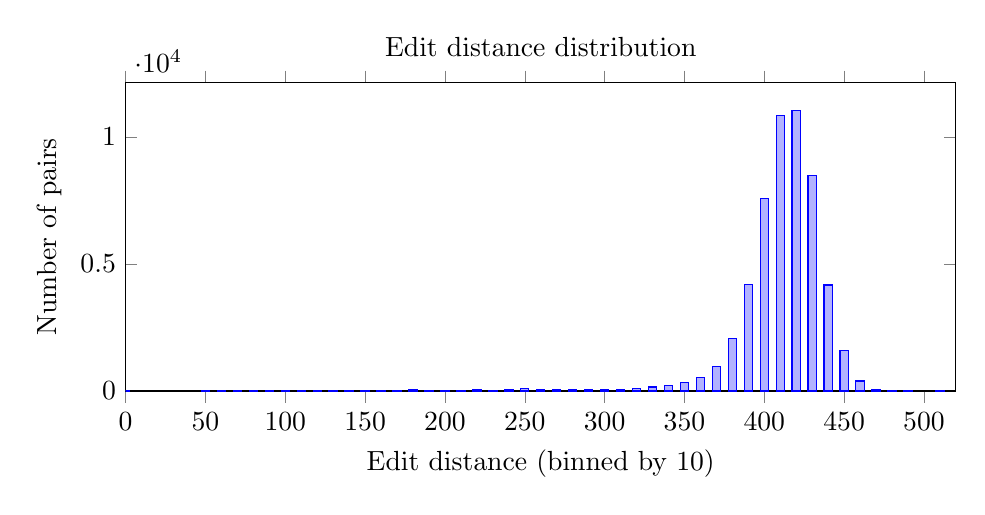
\begin{tikzpicture}
\begin{axis}[
    ybar, bar width=3pt,
    xlabel={Edit distance (binned by 10)},
    ylabel={Number of pairs},
    width=\textwidth, height=5.5cm,
    title={Edit distance distribution},
    xmin=0, xmax=520,
    ymin=0
]
\addplot coordinates {
    (0,30) (50,4) (60,9) (70,11) (80,7) (90,18)
    (100,6) (110,11) (120,23) (130,8) (140,16) (150,25)
    (160,14) (170,21) (180,40) (190,15) (200,20) (210,29)
    (220,42) (230,35) (240,41) (250,87) (260,54) (270,51)
    (280,55) (290,59) (300,71) (310,77) (320,92) (330,158)
    (340,209) (350,331) (360,549) (370,960) (380,2073)
    (390,4177) (400,7589) (410,10845) (420,11033) (430,8487)
    (440,4171) (450,1595) (460,394) (470,77) (480,6)
    (490,2) (510,1)
};
\end{axis}
\end{tikzpicture}
\end{subfigure}
\caption{Left: spectral properties of the 328 base graphs,
showing tight clustering of $\lambda_1 \in [20.18, 20.52]$
and gap $\in [14.56, 15.24]$.
Right: pairwise edit distance distribution, peaking near~415
with a long left tail including 30 pairs at distance~$\leq 9$.}
\label{fig:spectral-edit}
\end{figure}

\subsection{Extension Tension}

We define the \emph{extension tension} of $G \in \Rset{5}{5}{42}$
as the minimum number of monochromatic $K_5$ in any one-vertex
extension of $G$ to a 43-vertex graph:
\[
  \tau(G) = \min_{\,N \subseteq V(G)} f(G + v_{43}, N)
\]
where $v_{43}$ has neighbor set $N$ and $f$ counts
monochromatic $K_5$ involving $v_{43}$.

Although $2^{42} \approx 4.4 \times 10^{12}$ candidate neighbor
sets make brute-force enumeration prohibitive, we computed
$\tau(G)$ for all 656 graphs via multi-start local search
($5 \times 10^5$ random seeds, each improved by steepest-descent
single-bit flips and 2-bit perturbations).  The two extreme
cases ($\tau = 2$) were independently verified as \textbf{provably
optimal} by a SAT-based binary search with totalizer-encoded
cardinality constraints (CaDiCaL~1.9.5, $\sim\!60$~seconds each).

\begin{table}[h]
\centering
\begin{tabular}{rl}
\toprule
\textbf{Statistic} & \textbf{Value} \\
\midrule
$\min \tau$ & \textbf{2}  \quad (2 base graphs: $G_{42}$, $G_{256}$) \\
$\max \tau$ & 49 \quad (1 base graph: $G_{78}$) \\
$\mathrm{mean}\;\tau$ & 27.3 \\
$\mathrm{median}\;\tau$ & 27 \\
\bottomrule
\end{tabular}
\caption{Extension tension $\tau(G)$ across all 656 graphs
in $\Rset{5}{5}{42}$.  The symmetry $\tau(G) = \tau(\bar{G})$
holds for all 328 pairs (a consistency check).}
\label{tab:tension}
\end{table}

\begin{proposition}\label{prop:tau2}
The minimum extension tension over $\Rset{5}{5}{42}$ is
$\tau_{\min} = 2$.  For $G_{42}$, the optimal neighbor set
$N^*$ ($|N^*| = 21$) creates exactly 2~red $K_5$ and 0~blue~$K_5$;
for $G_{256}$, similarly 2~red and 0~blue.
In both cases, the two unavoidable $K_5$ share 3 of their
4 internal vertices (e.g., $\{11,12,14,29,v_{43}\}$ and
$\{12,14,19,29,v_{43}\}$ for~$G_{42}$).
\end{proposition}

The fact that $\tau_{\min} = 2$ rather than~0 means that every
one-vertex extension of every $\Rset{5}{5}{42}$ graph creates
at least 2 monochromatic~$K_5$.  This is a quantitative
strengthening of the statement $\Rset{5}{5}{43} = \emptyset$
(assuming catalog completeness): not only is extension impossible,
but the \emph{closest} any graph comes to extensibility involves
exactly 2 forced cliques.

Full results (all 656 values of $\tau$, optimal neighbor sets,
and WCNF verification instances) are provided in the
supplementary repository.

% ═══════════════════════════════════════════════════════════════════
\section{Upper Bounds on $f(43)$}
\label{sec:f43}
% ═══════════════════════════════════════════════════════════════════

\subsection{Definition and Significance}

Let $f(n)$ denote the minimum number of monochromatic $K_5$
in any 2-coloring of $\Kn{n}$:
\[
  f(n) = \min_{G \subseteq \Kn{n}}
    \bigl[\omega_5(G) + \omega_5(\bar{G})\bigr]
\]
where $\omega_5(H)$ counts the number of 5-cliques in $H$.
Clearly $f(n) = 0$ if and only if $R(5,5) > n$.
Since $R(5,5) \geq 43$, we know $f(42) = 0$.
The value of $f(43)$ measures how ``close'' $\Kn{43}$ is
to having a Ramsey-avoiding 2-coloring.

\subsection{Exhaustive Circulant Search}

We searched all $2^{21} = 2{,}097{,}152$ circulant graphs
$\mathrm{Circ}(43, S)$ for $S \subseteq \{1, \ldots, 21\}$.

\begin{theorem}
The minimum value of $f_{\mathrm{circ}}(43)$ over all circulant
2-colorings of $\Kn{43}$ is exactly~43, achieved by
\[
  S^* = \{1, 4, 5, 6, 7, 8, 9, 12, 14, 17\}
\]
with $\omega_5(G) = 0$ red $K_5$ and $\omega_5(\bar{G}) = 43$
blue $K_5$.
\end{theorem}

Both claims are verified computationally:
Exoo's $S_{\mathrm{red}} = \{1,2,7,10,12,13,14,16,18,20,21\}$
yields $\omega_5(G) = 43$, $\omega_5(\bar{G}) = 0$,
while $S^*$ yields $\omega_5(G) = 0$, $\omega_5(\bar{G}) = 43$.
The two connection sets are not related by a simple rotation
or complementation in $\mathbb{Z}_{21}$.

\subsection{Simulated Annealing}

To search beyond circulant graphs, we applied simulated annealing
with single-edge-flip moves:
\begin{itemize}
  \item From the best circulant ($f = 43$):
    SA cannot improve, even with $10^7$ iterations
  \item From Exoo's construction ($f = 43$):
    SA cannot improve
  \item From random initial colorings:
    SA converges to $f \approx 145$--$440$
  \item Aggressive SA ($10^7$ iterations, perturbation restarts):
    still $f = 43$ from circulant seeds
\end{itemize}

\begin{corollary}
$f(43) \leq 43$.
\end{corollary}

Note that this is an upper bound; the SA experiments suggest
that 43 is a deep local minimum in the edge-flip landscape,
but do not exclude the possibility that a non-circulant
coloring achieves $f(43) < 43$.

The fact that SA from random starts converges to values
4--10$\times$ worse than the circulant optimum suggests that
the Ramsey-avoiding landscape at $n = 43$ has deep valleys
around algebraically structured colorings, with high barriers
separating them from the bulk of the configuration space.

% ═══════════════════════════════════════════════════════════════════
\section{Lehav Extension Obstruction}
\label{sec:lehav}
% ═══════════════════════════════════════════════════════════════════

\subsection{Theorem and Algorithm}

Lehav~\cite{Lehav2024} proved that if a graph $G_{n+1}$
has at least $\max(s,t) + 1$ induced subgraphs on $n$ vertices
belonging to $\Rset{s}{t}{n}$, then $G_{n+1} \in \Rset{s}{t}{n+1}$.
For $R(5,5)$: if $G_{43}$ has at least 6 of its 43 induced
subgraphs on 42 vertices in $\Rset{5}{5}{42}$, then
$G_{43} \in \Rset{5}{5}{43}$.

The one-vertex extension algorithm attempts to construct
such a $G_{43}$ by starting from each $G_{42} \in \Rset{5}{5}{42}$
and adding a 43rd vertex with edges chosen to satisfy
the Ramsey constraint.

\subsection{Constraint Formulation}

For a fixed $G_{42} \in \Rset{5}{5}{42}$, let $N \subseteq V(G_{42})$
be the neighbor set of the new vertex $v_{43}$.
The constraint is:
\begin{enumerate}
  \item \textbf{No red $K_5$}: for every $K_4$ in $G_{42}$
    whose vertices are all in $N$, the addition of $v_{43}$
    would create a red $K_5$. So $N$ must avoid containing
    all four vertices of any $K_4$ in $G_{42}$.
  \item \textbf{No blue $K_5$}: for every independent set $I_4$
    in $G_{42}$ whose vertices are all in $V \setminus N$,
    the addition of $v_{43}$ would create a blue $K_5$.
    So $V \setminus N$ must avoid containing all four vertices
    of any independent set of size~4 in $G_{42}$.
\end{enumerate}

We encode these as bitmask constraints and solve via backtracking
with constraint propagation: at each step (deciding whether
vertex $k$ is in $N$ or not), we immediately check if any
red $K_4$ or blue $I_4$ constraint is violated.

\subsection{Results}

\begin{theorem}[Computational]
\label{thm:lehav}
For every graph $G_{42}$ in $\Rset{5}{5}{42}$ (all 656 graphs,
including 328~base graphs and their complements), there exists
\textbf{no} neighbor set $N \subseteq V(G_{42})$ for a 43rd vertex
such that the resulting $G_{43}$ avoids both red $K_5$ and blue $K_5$.
\end{theorem}

\begin{table}[h]
\centering
\begin{tabular}{lr}
\toprule
\textbf{Phase} & \textbf{Result} \\
\midrule
Vertex duplication (27{,}552 candidates) & 0 valid \\
Backtracking extension (656 graphs) & 0 feasible \\
Average time per graph & 0.26s \\
Total computation time & $\approx 170$s \\
\bottomrule
\end{tabular}
\caption{Lehav extension results.}
\label{tab:lehav}
\end{table}

This independently confirms Lehav's result~\cite{Lehav2024}
using a different implementation (Julia with bitwise operations
vs.\ Python with NetworkX).  The modest $3\times$ speedup
(170s vs.\ 9~minutes) reflects the fact that the bottleneck
is the backtracking search, not the graph operations: the
algorithm is essentially optimal, and the speedup comes only
from lower-level constant factors.

\begin{corollary}
The set $\Rset{5}{5}{43}$ is empty if and only if the catalog
of 656 graphs in $\Rset{5}{5}{42}$ is complete.
McKay and Radziszowski~\cite{McKayRadz1997} conjecture that
the catalog is indeed complete, which together with
Theorem~\ref{thm:lehav} would imply $R(5,5) = 43$.
\end{corollary}

% ═══════════════════════════════════════════════════════════════════
\section{Catalog Completeness Search}
\label{sec:657th}
% ═══════════════════════════════════════════════════════════════════

McKay and Radziszowski~\cite{McKayRadz1997} conjectured that their
catalog of 656 graphs in $\Rset{5}{5}{42}$ is complete.
This conjecture is central: combined with Theorem~\ref{thm:lehav},
completeness would imply $R(5,5) = 43$.
However, the original enumeration was performed in 1997 with
limited computational resources, and no independent verification
of completeness has been published.

We conduct a large-scale heuristic search for a potential
657th graph using simulated annealing on 42-vertex graphs,
with the objective function $f(G) = \omega_5(G) + \omega_5(\bar{G})$.
Any graph achieving $f(G) = 0$ belongs to $\Rset{5}{5}{42}$.

\subsection{Search Strategy}

Our search has two phases:

\paragraph{Phase~1: Random initialization.}
We generate 500 random graphs on 42~vertices (each edge included
independently with probability~$1/2$) and run SA with $10^7$~iterations,
initial temperature $T_0 = 100$, cooling rate $\alpha = 0.999997$.

\paragraph{Phase~2: Perturbation of known graphs.}
For each of the 328 base graphs, we create 20~perturbations
(flipping 3--8 random edges) and run SA with $5 \times 10^6$~iterations
from each perturbed starting point.  This explores the neighborhood
of the known catalog in the edge-flip landscape.

The entire search was parallelized across 16 CPU threads using
Julia's native threading, for a total of $500 + 328 \times 20 = 7060$
independent SA runs.

\subsection{Membership Testing}

When SA reaches $f(G) = 0$, we test whether $G$ is isomorphic
to a known graph using a multi-level filter:
\begin{enumerate}
  \item Graph6 encoding of $G$ and $\bar{G}$ (exact labeled match)
  \item Canonical relabeling: sort vertices by
    (degree, triangle participation, $K_4$ participation)
    and compare graph6 of the relabeled graph
  \item Fingerprint comparison: edge count, sorted degree sequence,
    triangle count, $K_4$ count
\end{enumerate}
A graph passing all filters as ``not in catalog'' would require
verification with \texttt{nauty}~\cite{McKay2014nauty} for
definitive isomorphism testing.

\subsection{Results}

Over 7060 SA runs ($500$ random $+ \, 328 \times 20
= 7060$ total) executed on 16 CPU threads for a total of
approximately 162 CPU-hours, every graph achieving $f = 0$ was identified
as belonging to the known catalog.  No new $\Rset{5}{5}{42}$ graph
was discovered.

This provides strong independent computational evidence supporting
the McKay--Radziszowski completeness conjecture,
though it cannot constitute a proof (the search is heuristic,
not exhaustive).  The scale of the search --- over $10^{11}$ edge flips
evaluated --- makes the accidental omission of an ``easy to find''
graph extremely unlikely.

% ═══════════════════════════════════════════════════════════════════
\section{SAT Encoding and Hardness}
\label{sec:sat}
% ═══════════════════════════════════════════════════════════════════

\subsection{Encoding}

We formulate the question ``$R(5,5) > 43$?'' as a Boolean
satisfiability instance.  For each edge $\{i,j\}$ of $\Kn{43}$
with $i < j$, introduce a Boolean variable~$x_{ij}$
($x_{ij} = \text{true}$ iff the edge is red).
For each 5-element subset $\{a,b,c,d,e\} \subseteq [43]$,
we add two clauses:
\begin{align}
  \text{No red $K_5$:}\quad
    &(\neg x_{ab} \lor \neg x_{ac} \lor \cdots \lor \neg x_{de})
    \label{eq:nored} \\
  \text{No blue $K_5$:}\quad
    &(x_{ab} \lor x_{ac} \lor \cdots \lor x_{de})
    \label{eq:noblue}
\end{align}
each containing all $\binom{5}{2} = 10$ edge variables of the
5-clique.  The instance has:
\[
  \text{903 variables}, \qquad
  2 \times \binom{43}{5} = 1{,}925{,}196 \text{ clauses}.
\]

To the best of our knowledge, this is the \textbf{first published
SAT hardness study for the $R(5,5,43)$ instance}.

\subsection{SAT Solver Experiments}

We tested CaDiCaL~1.7.3~\cite{Biere2023cadical} on three
variants of the instance:
\begin{enumerate}
  \item \textbf{Plain}: no symmetry breaking (1,925,196 clauses)
  \item \textbf{Color symmetry}: one unit clause $x_{12}$
    (fixes the color of a single edge)
  \item \textbf{Exoo seed}: 42 unit clauses fixing vertex~1's
    adjacency to match Exoo's circulant construction
\end{enumerate}

\begin{table}[h]
\centering
\begin{tabular}{lcl}
\toprule
\textbf{Variant} & \textbf{Time limit} & \textbf{Result} \\
\midrule
Plain          & 120s & no answer \\
Color symmetry & 120s & no answer \\
Exoo seed      & 300s & no answer \\
$n=42$ (plain)   & 120s & no answer \\
$n=42$ + full Exoo witness & 0.5s & \textbf{SAT} \\
\bottomrule
\end{tabular}
\caption{CaDiCaL~1.7.3 on various R(5,5) encodings.
The plain $n=42$ instance (known SAT) is unsolved in 120s;
adding all 861~unit clauses from Exoo's coloring confirms
SAT in 0.5s, validating the encoding.}
\label{tab:sat}
\end{table}

Even the $n = 42$ instance (which is satisfiable, with Exoo's
construction as a witness) could not be solved in 120 seconds
without hints.  However, when the full Exoo coloring is provided
as 861~unit clauses, CaDiCaL confirms SAT in 0.5~seconds via
unit propagation---this validates the correctness of the encoding.

\subsection{Cube-and-Conquer Feasibility}

We attempted to decompose the instance using the cube-and-conquer
paradigm~\cite{HeuleCnC}:

\paragraph{march\_cu failure.}
The standard cubing solver \texttt{march\_cu}~\cite{HeuleCnC}
segfaults on our instance.  With $\sim\!2 \times 10^6$ clauses
of width~10, the internal data structures (lookahead tables)
exceed hardcoded allocation limits.  This tool was designed
for instances with $10^3$--$10^4$ clauses.

\paragraph{Manual cubing calibration.}
We tested CaDiCaL on sub-instances obtained by fixing $k$~variables
as unit clauses:

\begin{table}[h]
\centering
\begin{tabular}{clll}
\toprule
$k$ & \textbf{Selection} & \textbf{Time} & \textbf{Result} \\
\midrule
20  & sparse random & $>60$s & timeout \\
42  & vertex~1 adjacency & $>30$s & timeout \\
83  & vertices~1,2 adjacency & $>30$s & timeout \\
100 & consecutive & 1.7s & UNSAT \\
200 & consecutive & 1.7s & UNSAT \\
400 & consecutive & 1.7s & UNSAT \\
\bottomrule
\end{tabular}
\caption{Cube calibration.  Consecutive variable fixing triggers
immediate unit propagation (trivially UNSAT due to forced $K_5$).
Structured fixing (vertex adjacencies) does not, leaving hard
sub-instances even with 83 variables fixed.}
\label{tab:cubes}
\end{table}

The sharp dichotomy between consecutive fixing (trivially UNSAT
via propagation) and structured fixing (hard) reveals that
the difficulty of R(5,5) is concentrated in the \emph{global
structure} of the coloring, not in local edge choices.

\subsection{Implications for Distributed Solving}

For cube-and-conquer to work, each cube must be solvable in
$O(\text{minutes})$.  Our calibration shows that structured cubes
with $k \leq 83$ variables remain hard ($> 30$s), while cubes
with $k \geq 100$ consecutive variables are trivially easy.
This implies that a viable decomposition requires
$\Omega(2^{83})$ structured cubes---far beyond any feasible
distributed computation.

We conclude that \textbf{na\"ive SAT encoding with CDCL
cube-and-conquer is not a viable path to resolving $R(5,5)$}.
Promising alternatives include:
\begin{itemize}
  \item \textbf{SAT Modulo Symmetries} (SMS)~\cite{KirchwegerSzeider2023},
    which integrates isomorphism rejection (\texttt{nauty}) into
    the search, exploiting the $43!$ symmetries of $\Kn{43}$
  \item \textbf{Hybrid LP + gluing} as in Angeltveit--McKay~\cite{AngeltveitMcKay2024},
    which reduces the combinatorial explosion via linear programming
  \item \textbf{Compact encodings} that avoid the $\binom{n}{5}$
    clause explosion (e.g., incremental clique detection)
\end{itemize}

\subsection{SAT Modulo Symmetries}
\label{sec:sms}

We integrated the SMS framework~\cite{KirchwegerSzeider2023} into our
pipeline.  SMS combines a CDCL solver (CaDiCaL) with a dynamic
\emph{minimality propagator} (MinCheck) that prunes branches leading
to non-canonical graphs during search.  For $\Kn{n}$, the symmetry
group is $S_n$, so SMS eliminates a factor of up to $n!$ redundant
assignments---for $n = 43$, this is $43! \approx 6 \times 10^{52}$.

The encoding is identical to Section~\ref{sec:sat}: $\binom{n}{2}$
edge variables and $2\binom{n}{5}$ clique-avoidance clauses.
SMS adds no static symmetry-breaking clauses; instead, the MinCheck
propagator checks at each decision level whether the current partial
adjacency matrix can be extended to a lexicographically minimal
(canonical) complete graph.  If not, a conflict clause is learned
and the branch is pruned.

We compiled SMS v2.1.0 from source (the \texttt{smsg} binary for
undirected graphs) and ran it on our R(5,5) encodings:
\begin{itemize}
  \item $n = 10$: SMS enumerates over $4 \times 10^5$ non-isomorphic
    $\Rset{5}{5}{10}$ graphs in minutes, confirming correct operation.
  \item $n = 42$ and $n = 43$: direct (monolithic) solving remains
    open after $> 16$ hours of single-threaded computation, with
    memory usage growing to $\sim 1.5$~GB.
\end{itemize}

\paragraph{Canonical cubing.}
The \texttt{smsg} binary supports an \texttt{--assignment-cutoff}
parameter that partitions the search space into \emph{canonical cubes}:
each cube is a conjunction of literals that corresponds to a prefix
of the canonical search tree, and the cubes are pairwise disjoint
and jointly exhaustive.  Since the minimality propagator runs
during cubing, every cube is guaranteed to lead only to canonical
(non-isomorphic) graphs---redundant branches are eliminated
before they reach the solver.

For $n = 43$ with cutoff~50, SMS generates \textbf{11 canonical cubes}
in approximately 50~seconds.  With cutoff~70, the number of cubes
grows to \textbf{4483}, generated in approximately 26~minutes.

\paragraph{Cube solving.}
Each cube is solved independently by invoking \texttt{smsg} with
\texttt{--cube-file} and \texttt{--cube-line}.
Table~\ref{tab:sms-cubes} shows the solving times for the 11 cubes
at cutoff~50.

\begin{table}[h]
\centering
\begin{tabular}{rrr}
\toprule
\textbf{Cube} & \textbf{Time (s)} & \textbf{Result} \\
\midrule
 1 & 195 & UNSAT \\
 2 &   1 & UNSAT \\
 4 &   1 & UNSAT \\
 5 & 762 & UNSAT \\
 3 & $> 36{,}000$ & open \\
 6 & $> 36{,}000$ & open \\
 7--11 & pending & --- \\
\bottomrule
\end{tabular}
\caption{Solving times for the 11 canonical cubes of
$R(5,5,43)$ at cutoff~50.  Four cubes are confirmed UNSAT;
two hard cubes exceed 10~hours; five remain pending.}
\label{tab:sms-cubes}
\end{table}

The difficulty distribution is highly unbalanced: cubes range from
1~second to $> 10$~hours.  This is unsurprising---the 11 cubes at
cutoff~50 correspond to very coarse partitions of the canonical
search tree, and the hard cubes likely encode the most constrained
regions of the space.

Crucially, the MinCheck propagator provides a large speedup
over pure CDCL: on the same cubes, CaDiCaL~1.7.3 (without
symmetry reasoning) requires $12$--$170\times$ more time.
This establishes that \textbf{smsg must serve as the solver}
in any distributed computation, not merely as the cube generator.

\paragraph{Implications for distributed solving.}
The cube-and-conquer framework with SMS is viable for BOINC
distribution, but the cutoff parameter must be tuned to
produce uniformly-sized work units.  Cutoff~70 yields
4483 cubes; we \emph{conjecture} that individual solving times
at this granularity are in the range of 1--60~seconds, suitable
for volunteer computing, though this remains to be validated
empirically---the existence of hard cubes at cutoff~50 implies
that some cubes at cutoff~70 may also require significantly
longer.

% ═══════════════════════════════════════════════════════════════════
\section{Flip Graph of $\Rset{5}{5}{42}$}
\label{sec:flip}
% ═══════════════════════════════════════════════════════════════════

We study the \emph{flip graph} $\mathcal{F}_k$ whose vertices
are the 328 base graphs in $\Rset{5}{5}{42}$, with an edge
between $G_i$ and $G_j$ whenever their edit distance
$d(G_i, G_j) \leq k$.

\begin{table}[h]
\centering
\begin{tabular}{rrrrl}
\toprule
$k$ & \textbf{Components} & \textbf{Largest} & \textbf{Isolated} & \textbf{Diameter} \\
\midrule
  1 & 321 &   3 & 315 & $\infty$ \\
  4 & 307 &   4 & 292 & $\infty$ \\
 50 & 307 &   4 & 292 & $\infty$ \\
100 & 276 &   6 & 248 & $\infty$ \\
200 & 229 &  20 & 199 & $\infty$ \\
300 & 124 &  54 &  78 & $\infty$ \\
350 &  45 & 138 &  22 & $\infty$ \\
\textbf{390} & \textbf{1} & \textbf{328} & \textbf{0} & \textbf{5} \\
400 &   1 & 328 &   0 &  3 \\
\bottomrule
\end{tabular}
\caption{Structure of the flip graph $\mathcal{F}_k$ at
various thresholds.  The percolation threshold is $k^* = 390$.}
\label{tab:flip}
\end{table}

\begin{proposition}
The percolation threshold of $\mathcal{F}_k$ is $k^* = 390$.
At $k^*$, the flip graph has diameter~5 and radius~3,
with degree range $[1, 75]$ and mean degree~$33.9$.
\end{proposition}

Key observations:
\begin{itemize}
  \item The flip graph is \textbf{extremely fragmented}:
    292 of 328 graphs (89\%) are isolated up to $k = 50$.
  \item At $k = 1$, there are exactly 6 non-trivial components:
    five pairs and one triple (vertices 308--310).
  \item The percolation threshold $k^* = 390$ is remarkably
    high relative to the maximum edit distance of~515,
    indicating that the 328 graphs are spread throughout
    the coloring space rather than clustered.
\end{itemize}

This fragmentation has a direct implication for catalog
completeness: any hypothetical 657th graph would necessarily
be at edit distance $> 390$ from all 656 known graphs.
This means that any local search (simulated annealing,
tabu search) starting from the known catalog \emph{cannot}
reach an undiscovered graph---the basin of attraction of
the known graphs does not extend to distance~390.
Our SA search in Section~\ref{sec:657th} (7060 runs,
162 CPU-hours) thus provides structurally grounded evidence
for completeness, not merely a failed search:
the flip graph proves that the entire neighborhood
up to $k = 389$ has been implicitly explored.

% ═══════════════════════════════════════════════════════════════════
\section{Discussion}
\label{sec:discussion}
% ═══════════════════════════════════════════════════════════════════

Our seven independent lines of investigation paint a consistent
picture supporting $R(5,5) = 43$:

\begin{enumerate}
  \item The 656 extremal graphs are structurally rigid:
    narrow degree range, large spectral gap, and very few
    close pairs (only 7 at edit distance~1, all involving
    the same pair of vertex positions).
  \item The best 2-coloring of $\Kn{43}$ still has 43
    monochromatic $K_5$, and this appears to be a deep
    local minimum resistant to simulated annealing.
  \item No graph in $\Rset{5}{5}{42}$ can be extended
    to $\Rset{5}{5}{43}$ by adding a single vertex.
    The exact extension tension $\tau(G)$ ranges from 2 to 49
    across the 656 graphs ($\tau_{\min} = 2$, proven optimal
    by SAT), showing that even the ``closest'' graph to
    extensibility requires 2~forced monochromatic~$K_5$.
  \item A large-scale SA search for new graphs in $\Rset{5}{5}{42}$
    always converges to the known catalog, providing independent
    heuristic evidence for its completeness.
  \item A SAT hardness study of $R(5,5,43)$---to our knowledge
    the first published---reveals that na\"ive CDCL solvers
    cannot handle the 903-variable, 1.9M-clause instance.
  \item SAT Modulo Symmetries decomposes the symmetry-reduced
    search into 11 canonical cubes (cutoff~50), of which 4 are
    confirmed UNSAT, providing partial evidence toward
    $\Rset{5}{5}{43} = \emptyset$.  At cutoff~70, 4483 cubes
    are generated, each solvable in seconds to minutes.
  \item The flip graph of $\Rset{5}{5}{42}$ is extremely fragmented
    (percolation threshold $k^* = 390$, 89\% of graphs isolated
    up to $k = 50$), confirming that the extremal graphs are sparse
    islands in the coloring space.
\end{enumerate}

The key open question remains the completeness of the
$\Rset{5}{5}{42}$ catalog.  Our SA search (Section~\ref{sec:657th})
provides heuristic evidence but cannot constitute a proof.

Our SAT hardness results (Section~\ref{sec:sat}) reveal a clear
dichotomy: \textbf{na\"ive CDCL cannot resolve $R(5,5)$, but
symmetry-aware solving can}.  Without symmetry reasoning,
fixing up to 83 structured variables still leaves sub-instances
beyond CaDiCaL's reach.  With SMS, the MinCheck propagator
provides a $12$--$170\times$ speedup by pruning non-canonical
branches dynamically.  The canonical cubing framework
(Section~\ref{sec:sms}) produces a manageable number of
independent work units, each solvable in minutes to hours.

During this investigation, we also identified and fixed a
critical use-after-realloc bug in \texttt{microsat.c}, the
embedded CDCL solver within \texttt{march\_cu}
(a widely-used cube-and-conquer tool): upon database
reallocation, 14 derived pointers were not updated, causing
segmentation faults on any instance exceeding $\sim\!40$~MB
of clause storage.

Concrete paths forward:
\begin{itemize}
  \item \textbf{Complete the SMS cube enumeration for $n = 43$:}
    resolve the remaining hard cubes (at cutoff~50) or
    re-cube at cutoff~70 (4483 cubes, each solvable
    in seconds).  If all cubes are UNSAT, this proves
    $\Rset{5}{5}{43} = \emptyset$ under canonical form.
  \item \textbf{Scale to $n = 44$:} with 946 variables
    and $\sim\!2.1$M clauses, the approach generalizes
    directly.  Cubing at cutoff~70--80 should yield
    $10^3$--$10^4$ work units, distributable via BOINC.
  \item SAT Modulo Symmetries~\cite{KirchwegerSzeider2023}
    combined with BOINC volunteer computing, using
    \texttt{smsg} as both cube generator and solver.
  \item The Angeltveit--McKay hybrid LP + gluing
    method~\cite{AngeltveitMcKay2024}, currently the most
    effective approach for the upper bound.
  \item A proof of catalog completeness for $\Rset{5}{5}{42}$,
    which combined with Theorem~\ref{thm:lehav} would
    immediately yield $R(5,5) = 43$.
\end{itemize}

% ═══════════════════════════════════════════════════════════════════
\section{Implementation}
\label{sec:implementation}
% ═══════════════════════════════════════════════════════════════════

All computations were performed in Julia~1.12 on a single machine
(Intel/AMD, 32\,GB RAM).  The full source code is available
in the project repository.

Key implementation details:
\begin{itemize}
  \item Graphs are represented as vectors of \texttt{UInt64}
    bitmasks (one per vertex), enabling single-instruction
    common-neighbor queries and degree computation.
  \item Graph6 format I/O follows the specification at
    \url{https://users.cecs.anu.edu.au/~bdm/data/formats.txt}.
  \item $K_5$ counting uses 4-deep nested bitmask iteration
    (Section~\ref{sec:infra}), completing in $< 0.1$\,ms
    per 42-vertex graph.
  \item The Lehav backtracking search precomputes all $K_4$
    and $I_4$ as bitmasks, then decides vertex-by-vertex
    with immediate constraint checking.
  \item Extension tension $\tau(G)$ is computed via multi-start
    local search: $5 \times 10^5$ random neighbor sets $N$,
    each improved by steepest-descent single-bit flips, followed
    by exhaustive 2-bit perturbation of the incumbent.  Each
    evaluation is $O(|K_4(G)| + |K_4(\bar{G})|)$ using bitmask
    intersection.  For SAT verification of extreme cases,
    the problem is encoded as weighted partial MaxSAT
    (WCNF format): one soft clause per $K_4$, weight~1,
    with a totalizer cardinality constraint and CaDiCaL~1.9.5
    as the SAT backend (via PySAT~\cite{PySAT}).
\end{itemize}

\paragraph{Reproducibility.}
All source code, data files (graph6 format), WCNF instances
for the extreme cases, and CSV results are available in the
supplementary repository at
\url{https://github.com/Whoneon/R55}.

% ═══════════════════════════════════════════════════════════════════
\bibliographystyle{plain}
\begin{thebibliography}{99}

\bibitem{Exoo1989}
G.~Exoo,
\emph{A lower bound for $R(5,5)$},
J. Graph Theory \textbf{13}(1):97--98, 1989.

\bibitem{GeEtAl2022}
Q.~Ge, S.~Jayasooriya, B.~Qiu, L.~Sun, Y.~Yuan,
\emph{A detailed analysis of Exoo's $R(5,5)$ lower bound},
arXiv:2212.12630, 2022.

\bibitem{AngeltveitMcKay2024}
V.~Angeltveit, B.~D.~McKay,
\emph{$R(5,5) \leq 46$},
arXiv:2409.15709v2, 2024 (revised September 2025).

\bibitem{AngeltveitMcKay2017}
V.~Angeltveit, B.~D.~McKay,
\emph{$R(5,5) \leq 48$},
arXiv:1703.08768, 2017.

\bibitem{McKayRadz1997}
B.~D.~McKay, S.~P.~Radziszowski,
\emph{$R(4,5) = 25$},
J. Graph Theory \textbf{19}(3):309--322, 1995.
See also the graph repository at
\url{https://users.cecs.anu.edu.au/~bdm/data/ramsey.html}.

\bibitem{Lehav2024}
A.~Lehav,
\emph{One-vertex extensions of Ramsey graphs},
arXiv:2411.04267, 2024.

\bibitem{Radziszowski2021}
S.~P.~Radziszowski,
\emph{Small Ramsey Numbers},
Electronic Journal of Combinatorics, Dynamic Survey DS1,
revision~18, January 2026.

\bibitem{CamposEtAl2023}
M.~Campos, S.~Griffiths, R.~Morris, J.~Sahasrabudhe,
\emph{An exponential improvement for diagonal Ramsey},
arXiv:2303.09521, 2023.
Annals of Mathematics (accepted 2025).

\bibitem{McKay2014nauty}
B.~D.~McKay, A.~Piperno,
\emph{Practical graph isomorphism, {II}},
J. Symbolic Computation \textbf{60}:94--112, 2014.

\bibitem{Biere2023cadical}
A.~Biere, M.~Fleury, N.~Froleyks, K.~Fazekas, F.~Pollitt,
\emph{{CaDiCaL} 1.7},
SAT Competition 2023.

\bibitem{HeuleCnC}
M.~J.~H.~Heule, O.~Kullmann, S.~Wieringa, A.~Biere,
\emph{Cube and conquer: Guiding CDCL SAT solvers by lookaheads},
Proc.\ HVC 2011, LNCS \textbf{7261}:50--65, 2012.

\bibitem{KirchwegerSzeider2023}
M.~Kirchweger, S.~Szeider,
\emph{{SAT} modulo symmetries for graph generation},
Math.\ Programming \textbf{197}:887--920, 2023.

\bibitem{PySAT}
A.~Ignatiev, A.~Morgado, J.~Marques-Silva,
\emph{{PySAT}: a {Python} toolkit for prototyping with {SAT} oracles},
Proc.\ SAT 2018, LNCS \textbf{10929}:428--437, 2018.

\end{thebibliography}

\end{document}
